\documentclass[a4paper,12pt]{article} % тип документа

\usepackage{tikz}
\usepackage[T2A]{fontenc}			% кодировка
\usepackage[utf8]{inputenc}			% кодировка исходного текста
\usepackage[english,russian]{babel}	% локализация и переносы
\usepackage{amsfonts,longtable}

% Математика
\usepackage{amsmath,amsfonts,amssymb,amsthm,mathtools} 


\usepackage{wasysym}

\title{Лабораторная работа 1.2.1 по курсу \\ "Общая физика"  \\ 
\vspace{0.2cm}
\vspace{4.5cm}
 \LARGE{\textbf{Определение скорости полета пули при помощи баллистического маятника}}\vspace{5.5cm}}
\date{19.10.2018}
\usepackage{tikz}
\author{\vspace{0.2cm}Баринов Леонид}

\begin{document}

\maketitle

\newpage

\section{Аннотация} В работе будет определена скорость полета пули с помощью воздействия пули на баллистические маятники

\section{Теоритические сведения}
Для измерения переданного пулей импульса и, следовательно, ее скорости используют баллистический маятник. Баллитическим называется маятник, колебания которого вызываются кратковременныи начальным импульсом (толчком). Кратковременным можно считать импульс, если время действия сил (время соударения) значительно меньше периода колебаний маятника. При этом отклонение маятника за время соударения значительно меньше амплитуды колебаний - максимальное время соударения $\tau$, отнесенное к периоду колебаний $T$, и отклонение $\Delta\varphi$ за время соударения, отнесенное к максимальному отклонению $\Delta_m$ (амплитуде), связаны простым соотношением
\[\frac{\Delta\varphi}{\varphi_m}\approx\frac{2\pi\tau}{T}\]
Влияние струи газов на маятник можно оценить с помощью холостого выстрела. Ружье закреплено на специальном штативе. Чтобы зарядить ружье, надо освободить стопорный винт штатива и наклонить ружье в держателе набок. Затем отогнуть ствол в сторону курка до упора. Зарядив ружье, все вернуть в первоначальное состояние.
\begin{figure}[h]
\centering
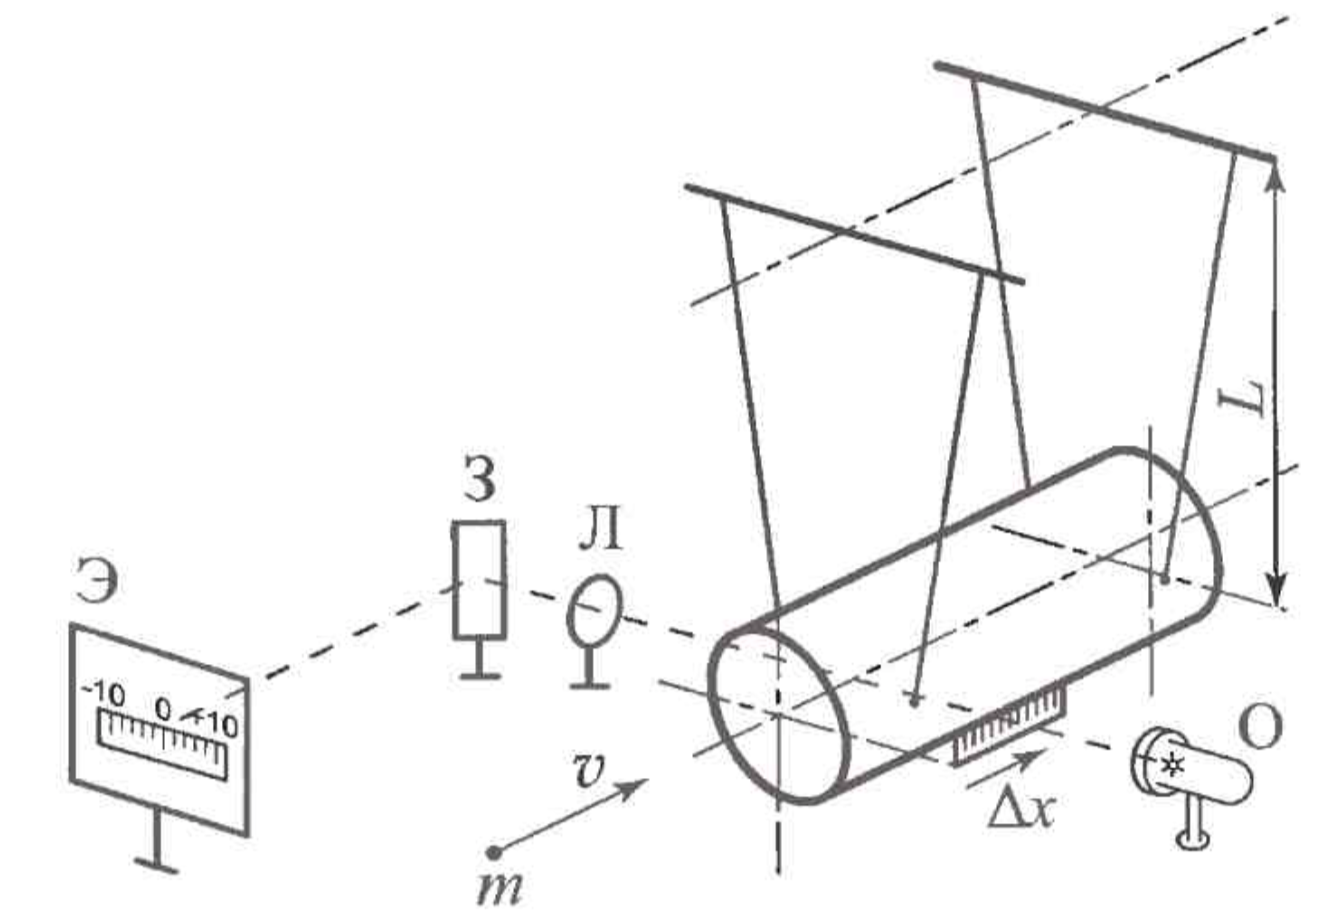
\includegraphics[scale = 0.4]{1}
\caption{Схема установки для измерения скорости полета пули}
\end{figure}
\newpage

\subsection{Метод баллистического маятника, совершающего поступательное движение}
Используемый в этой части работы баллистической маятник представляет собой тяжелый цилиндр, подвешенный на четерых нитях одинаковой длины. Он изображен на Рис. 1 вместе в измерительной системой.

Закон сохранения импульса при соударении пули с цилиндром имеет вид
\begin{equation}
mu = (M+m)V
\end{equation}
Здесь $m$ -- масса пули, $M$ -- масса цилиндра, $u$ -- скорость пули перед ударом, $V$ -- скорость цилиндра и пули после неупругого соударения.

Учитывая, что масса маятника значительно больше массы пули, можно написать
\begin{equation}
u = \frac{M}{u}V
\end{equation}
Получив начальную кинетическую энергию, маятник при отклонении будет подниматься до тех пор, пока всю ее не израсходует. Если пренебречь потерями, то вся кинетическая энергия переходит в потенциальную в поле тяжести. Тогда по закону сохранения механической энергии высота $h$ подъема маятника над его начальным положением связана с начальной скоростью маятника $V$ следующим образом:
\begin{equation}
V^2=2gh
\end{equation}
Здесь $g$ - ускорение свободного падения.

Высота подъема маятника выражается через угол $\varpi$ отклонения маятника от вертикали:
\begin{equation}
\begin{aligned}
h = L(1-cos\varphi) = 2Lsin^2\frac{\varphi}{2}, & & где \varphi\approx\frac{\Delta x}{L}\\
\end{aligned}
\end{equation}
Из (2), (3) и (4) получаем окончательную формулу для определения скорости пули:
\begin{equation}
u = \frac{M}{m}\sqrt{\frac{g}{L}}\Delta x
\end{equation}
\begin{figure}[h]
\centering
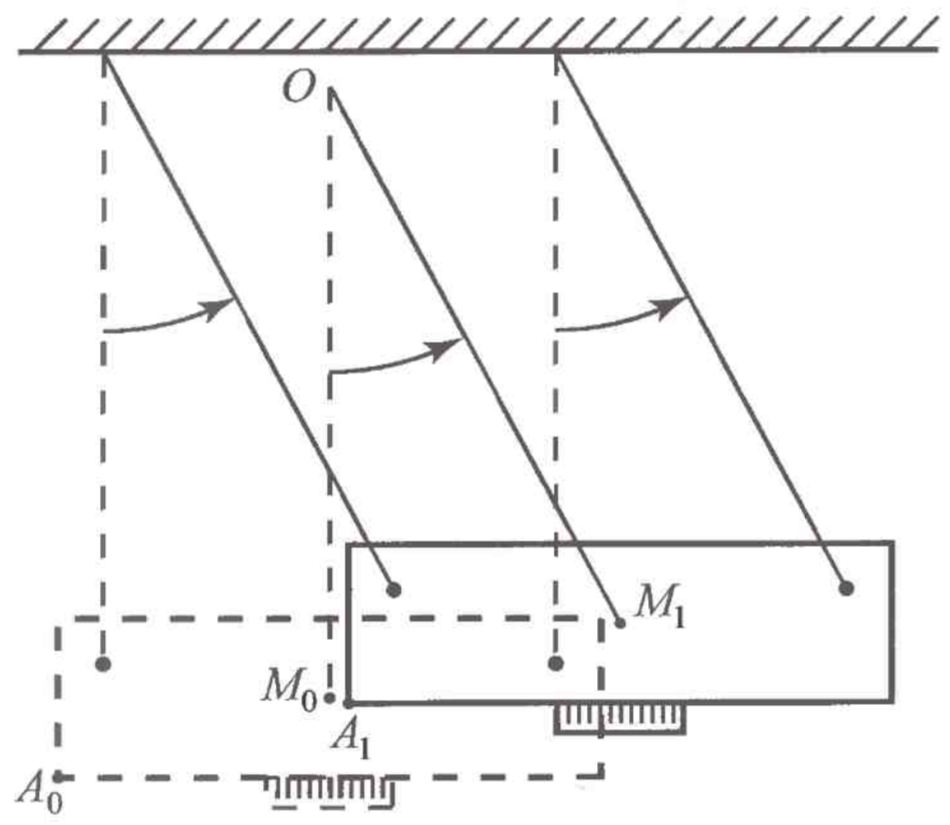
\includegraphics[scale = 0.4]{2}
\caption{Схема установки для измерения скорости полета пули}
\end{figure}
\subsection{Метод крутильного баллистического маятника}
Схема эксперимента изображена на Рис. 3. Пуля массой $m$ попадает в мишень, укрепленную на стержне $aa$, который вместе с грузами $M$  и проволкой П образует крутильный маятник.
\begin{figure}[h]
\centering
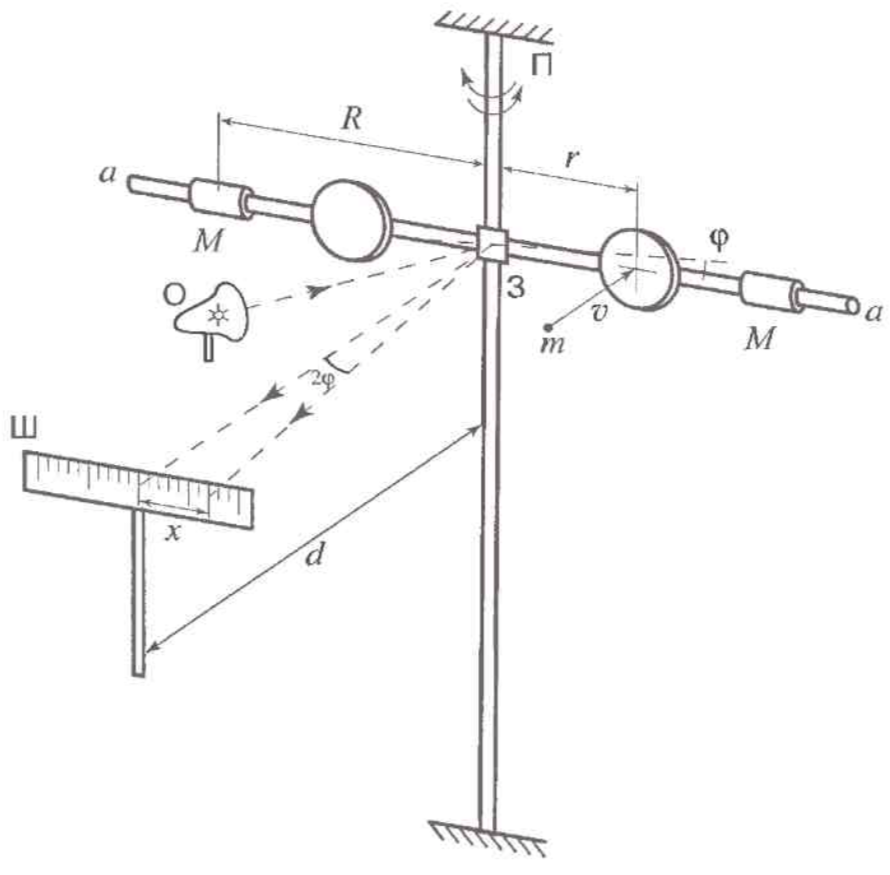
\includegraphics[scale = 0.4]{3}
\caption{Схема установки для измерения скорости полета пули}
\end{figure}
 Считая удар пули о мишень неупругим, для определения скорости $u$ полета пули непосрдественно перед ударом воспользуемся законом сохранения момента импульса в виде
 \begin{equation}
 mur=I\Omega
 \end{equation}
 Здесь $r$ -- расстояние от линии полета пули до оси вращения маятника (до проволки П), $I$ -- момент инерции маятника, $\Omega$ -- его угловая скорость непосредственно после удара.
 
 Пренебрегая потерями, закон сохранения энергии при колебаниях записываем следующим образом:
 \begin{equation}
 k\frac{\varphi^2}{2}=I\frac{\Omega^2}{2}
 \end{equation}
 Здесь $k$ -- модуль кручения проволки П, а $\varphi$ -- максимальный угол поворота маятника.
 
Из (6) и (7) получаем
\begin{equation}
u = \varphi\frac{\sqrt{kI}}{mr}
\end{equation}
Угол максимального закручивания маятника в данных опытах всегда мал и легко находится по смещения $x$ изображения нити освитетля на измерительной шкале. Из Рис. 3 следует
\begin{equation}
\varphi\approx\frac{x}{2d}
\end{equation}
Здесь $d$ - расстояние от шкалы Ш до оси вращения маятника.

В формулу (8) входит проивзедения $kI$, которое можно найти по измерениям периодов колебаний мфятника с грузами $M$ и без них. В первом случае период колебаний равен:
\begin{equation}
T_1 = 2\pi\sqrt{\frac{I}{k}}
\end{equation}
Во втором случае
\begin{equation}
T_2 = 2\pi\sqrt{\frac{I-2MR^2}{k}}
\end{equation}
Из (10) и (11) следует
\begin{equation}
\sqrt{kI}=\frac{4\pi MR^2T_1}{T_1^2-T_2^2}
\end{equation}
Здесь $R$ -- расстояние от центров массс грузов $M$ до проволки.
\newpage
\section{Оборудование и инструментальные погрешности}
Для измерения массы пулек использовались электронные весы. 
\[\sigma_{1\text{сист}} = 0,01\text{г}\]
Систематическая погрешность измерения координаты $x$ в опыте с 1-ой установкой (Рис. 1, Рис. 2):
\[\sigma_{x_1} = 0,25\text{мм}\]
Систематическая погрешность измерения координаты $x$ в опыте со 2-ой установкой (Рис. 3):
\[\sigma_{x_2} = 1\text{см}\]
Систематическая погрешность измерения расстояния $L$ :
\[\sigma_{L\text{сист}} = 1\text{мм}\]
Указанная на цилндре его масса в опыте с 1-ой установкой (Рис. 1, Рис. 2):
\[M = 2905\pm5\text{г}\]
Указанные на цилиндрах их масса в опыте с 2-ой установкой (Рис. 3):
\[
\begin{aligned}
M_1 = 724,5\text{г}; & & M_2 = 725,8\text{г}\\
\end{aligned}
\]
Измерения $r_1$, $r_2$, $R_1$, $R_2$, $d$ проводилоись одной и той же линейкой с систематической погрешностью:
\[\sigma_{2\text{сист}} = 1 \text{мм}\]
\section{Результаты измерений и обработка данных}

Измеряем массу 8 пулек. В 1-ом опыте используются пули c $\text{№}$ от 1 до 4, во втором с $\text{№}$ от 5 до 8. Результаты измерений занесем в Таблицу 1.
\newpage
\begin{table}[h]
\centering
\caption{Измерение массы пулек}
\begin{tabular}{|c|c|c|c|c|}
\hline
$\text{№}$  & 1 & 2 & 3 & 4  \\ \hline
$m$, г & 0,523 & 0,521 & 0,526 & 0,510 \\ \hline \hline
$\text{№}$  & 5 & 6 & 7 & 8  \\ \hline
$m$, г & 0,524 & 0,507 & 0,520 & 0,510 \\ \hline 
\end {tabular}
\end {table}
\textbf{Метод баллистического маятника, совершающего поступательное движение}

Измеряем расстояние $L$ для каждой из точек крепления маятника. Результаты измерений запишем в Таблицу 2.
\begin{table}[h]
\centering
\caption{Измерение длины нити крепления маятника}
\begin{tabular}{|c|c|c|c|c|}
\hline
$\text{№}$  & 1 & 2 & 3 & 4  \\ \hline
$L$, см & 220 & 219 & 220 & 220 \\ \hline
\end {tabular}
\end {table}
\[\overline L = \frac{1}{N}\sum_{i=1}^NL_i = 219,75 \text{см}\]
Найдем среднеквадратичную ошибку отдельного измерения:
\[\sigma_L = \sqrt{\frac{1}{N}\sum_{i=1}^N(L_i-\overline{L})^2} \approx 0,43\text{см}\]
Найдем срендеквадратичную ошибку $\overline{L}$:
\[\sigma_{\overline L} = \frac{\sigma_L}{\sqrt{N}}\approx 0,22\text{см}\]
Найдем погрешность $L$:
\[\sigma_L = \sqrt{\sigma_{\overline{L}}^2+\sigma_{L\text{сист}}^2}\approx0,24\text{см}\]
Собирем оптическую систему, предзназначенную для измерения перемещения маятника. Включем осветитель и добиваемся четкого изображения шкалы на экране. Начальная координата на шкале: \[x_0 = 2.00\pm0.25\text{мм}\]

Произведем несколько холостых выстрелов по маятнику и убеждаемя в том, что она практически не реагирует на удары воздушной струи из ружья.
\newpage
Убедимся в малом затухании колебаний: за десть колебаний амплитуда уменьшается меньше, чем наполовину.

Произведем несколько выстрелов и измеряем координату максимального отклонения. Находим $\Delta x = x_1-x_0$. Резульаты заносим в Таблицу 3.

\begin{table}[h]
\caption{Амплитуда колебаний маятника}
\centering
\begin{tabular}{|c|c|}
\hline
$x_1$, мм & $\Delta x$, мм \\ \hline
8,25 & 6,25 \\ \hline
8,5 & 6,5\\ \hline
9 & 7\\ \hline
9,5 & 7,5\\ \hline
\end{tabular}
\end{table}
\[\sigma_{\Delta_x} = \sigma_{x_0} + \sigma_{x_1} = 0,25\text{мм}+0,25\text{мм} = 0,5\text{мм}\]
Определим по формуле (5) скорость пули при каждом выстреле.\[u = \frac{M}{m}\sqrt{\frac{g}{L}}\Delta x\] Находим $\sigma u$ по формуле:
\[\sigma u = u\sqrt{\left(\frac{\sigma_M}{M}\right)^2+\left(\frac{1}{2}\right)^2\left(\frac{\sigma_L}{L}\right)^2+\left(\frac{\sigma_{\Delta_x}}{\Delta x}\right)}\]
Результаты заносим в таблицу 4.


\begin{table}[h]
\centering
\caption{Измерение скорости полета пули}
\begin{tabular}{|c|c|c|}
\hline
$\text{№}$ & $u$, м/с & $\sigma$, м/с \\ \hline
1 & 74,06 & 5,93\\ \hline
2 & 77,31& 5,95\\ \hline
3& 82,47& 5,89\\ \hline
4 & 91,13& 6,08\\ \hline
\end{tabular}
\end{table}
Найдем среднее значение скорости пули:
\[u_\text{ср} = \frac{1}{N}\sum_{i=1}^{N}u_i = 81,24\text{м/с}\]
Найдем среднеквадратичную ошибку отдельного измерения:
\[\sigma_u = \sqrt{\frac{1}{N}\sum_{i=1}^N(u_i-\overline{u})^2} \approx 6,44\text{м/c}\]
Найдем срендеквадратичную ошибку ${u_\text{ср}}$:
\[\sigma_{u_\text{ср}} = \frac{\sigma_u}{\sqrt{N}}\approx 3,22\text{м/c}\]
Итого получаем:
\[u = u_\text{ср}\pm\sigma_{u_\text{ср}} = (81,24\pm3,22)\text{м/с}\]

\textbf{Метод крутильного баллистического маятника}

Измеряем с помощью линейки расстояния $r_1, r_2, R_1, R_2, d$. Результаты занесем в Таблицу 5.
\begin{table}[h]
\centering
\caption{Измерение расстояний с помощью линейки}
\begin{tabular}{|c|c|}
\hline
$r_1$ & $20,5\text{см}$ \\ \hline
$r_2$& $21,5\text{см}$\\ \hline
$R_1$ & $34\text{см}$\\ \hline
$R_2$& $33,5\text{см}$\\ \hline
$d$ & $34\text{см}$\\ \hline
\end{tabular}
\end{table}

\[\overline{r}= \frac{r_1+r_2}{2} = 21\text{см}\]
\[\sigma_{\overline{r}} = 2\text{мм}\]
\[\overline{R}= \frac{R_1+R_2}{2} = 33,75\text{см}\]
\[\sigma_{\overline{R}} = 2\text{мм}\]
\[\overline{M}= \frac{M_1+M_2}{2} = 725,15\text{г}\]
Настроим оптическую систему, предназначенную для измерения проворота маятника. Включаем осветитель О, направим свет на зеркальце З и получаем четкое изображение нити осветителя на шкале. Начальная координата $x_0 = 3.5\text{см}$

Произведем несколько холостых выстрелов и убедимся, что маятник практически не реагирует на воздушную струю из ружья.

Убеждаемся в малом затухании колебаний: за десять колебаний амплитуда уменьшается меньше, чем наполовину.

Измеряем время 10 полных крутильных колебаний маятника.Определяем $T_1$ и $T_2$, как отношение времени колебаний маятника к количеству колебаний. Результаты заносим в Таблицу 6:
\begin{table}[h]
\centering
\caption{Измерение перода колебаний}
\begin{tabular}{|c|c|c|c|c|}
\hline
$\text{№}$ & $t_1$, c & $T_1$, c & $t_2$, c & $T_2$, c\\ \hline
1 & 166,93 & 16,69 & 130,82 & 13,08\\ \hline
2 & 172,24 & 17,22 & 122,67 & 12,27\\ \hline
3& 170, 81 & 17,08 & 125,5 & 12,55\\ \hline
\end{tabular}
\end{table}
Найдем среднее значение перода колебаний маятника без грузиков:
\[\overline{T_1} = \frac{1}{N}\sum_{i=1}^{N}T_1 \approx 17\text{с}\]
Найдем среднеквадратичную ошибку отдельного измерения:
\[\sigma_{T_1} = \sqrt{\frac{1}{N}\sum_{i=1}^N(T_1-\overline{T_1})^2} \approx 0,22\text{c}\]
Найдем срендеквадратичную ошибку ${u_\text{ср}}$:
\[\sigma_{\overline{T_1}} = \frac{\sigma_{T_1}}{\sqrt{N}}\approx 0,13\text{c}\]

Найдем среднее значение перода колебаний маятника c грузикaми:
\[\overline{T_2} = \frac{1}{N}\sum_{i=1}^{N}T_2 \approx 12,63\text{с}\]
Найдем среднеквадратичную ошибку отдельного измерения:
\[\sigma_{T_2} = \sqrt{\frac{1}{N}\sum_{i=1}^N(T_2-\overline{T_2})^2} \approx 0,34\text{c}\]
Найдем срендеквадратичную ошибку ${u_\text{ср}}$:
\[\sigma_{\overline{T_2}} = \frac{\sigma_{T_2}}{\sqrt{N}}\approx 0,2\text{c}\]


По формуле (12) найдем величину $\sqrt{kI}$ и оценим ее погрешность:
\[\sqrt{kI}=\frac{4\pi MR^2T_1}{T_1^2-T_2^2} = 0,14\frac{\text{кг}\cdot \text{м}^2}{c}\]
\[\sigma_{\overline{T_1}^2} = 2\sigma_{\overline{T_1}} = 0,26\text{c}\]
\[\sigma_{\overline{T_2}^2} = 2\sigma_{\overline{T_2}} = 0,68\text{c}\]
\[\sigma_{\overline{T_1}^2-\overline{T_2}^2}  = \sigma_{\overline{T_1}^2}+\sigma_{\overline{T_2}^2}=0,94\text{c}\]
\[\sigma_{\overline{R}^2} = 2\sigma_{\overline{R}} = 4\text{мм}\]
\[\sigma_{\sqrt{kI}} = \sqrt{kI} \sqrt{\left(\frac{\sigma_M}{M}\right)^2+\left(\frac{\sigma_{R^2}}{R^2}\right)^2 + \left(\frac{\sigma_{T_1}}{T_1}\right)^2 + \left(\frac{\sigma_{\overline{T_1}^2-\overline{T_2}^2}}{\overline{T_1}^2-\overline{T_2}^2}\right)^2} = 0,015\frac{\text{кг}\cdot \text{м}^2}{c} \]

Произведем несколько выстрелов и измеряем координату максимального отклонения. Находим $\Delta x = x_1-x_0$. Резульаты заносим в Таблицу 7.
\begin{table}[h]
\caption{Амплитуда колебаний маятника}
\centering
\begin{tabular}{|c|c|}
\hline
$x_1$, cм & $\Delta x$, cм \\ \hline
9 & 5,5 \\ \hline
10,5 & 6,5\\ \hline
9,5 & 5,5\\ \hline
10,5 & 6,5\\ \hline
\end{tabular}
\end{table}
\[\sigma_{\Delta_x} = \sigma_{x_0} + \sigma_{x_1} = 1\text{cм}+1\text{cм} = 2\text{cм}\]
Посчитаем угол максимального закручивания маятника по формуле (9) и его погрешность . Результаты занесем в таблицу 8. 
\[\sigma_{\varphi} = \varphi\left(\frac{\sigma_{\Delta x}}{\Delta x}\right)\]
\begin{table}[!h]
\caption{Угол максимального закручиваниы маятника}
\centering
\begin{tabular}{|c|c|c|}
\hline
$\text{№}$ & $\varphi$ & $\sigma_\varphi$ \\ \hline
1 & 0,08 & 0,03\\ \hline
2 & 0,1 & 0,03\\ \hline
3 & 0,08 & 0,03\\ \hline
4 & 0,1 & 0,03\\ \hline
\end{tabular}
\end{table}
\newpage
Определим скорость пули при каждом выстреле по формуле (8) и ее погрешность. Результаты занесем в Таблицу 9.
\[\sigma_u = u\sqrt{\left(\frac{\sigma_{\varphi}}{\varphi}\right)^2+\left(\frac{\sigma_{\sqrt{kI}}}{\sqrt{kI}}\right)^2+\left(\frac{\sigma_r}{r}\right)^2}\]
\begin{table}[h]
\centering
\caption{Измерение скорости полета пули}
\begin{tabular}{|c|c|c|}
\hline
$\text{№}$ & $u$, м/с & $\sigma$, м/с \\ \hline
1 & 101,78 & 39,7\\ \hline
2 & 131,5& 41,9\\ \hline
3& 102,56 & 40\\ \hline
4 & 130,72 & 41,7\\ \hline
\end{tabular}
\end{table}
Найдем среднее значение скорости пули:
\[u_\text{ср} = \frac{1}{N}\sum_{i=1}^{N}u_i = 116,64\text{м/с}\]
Найдем среднеквадратичную ошибку отдельного измерения:
\[\sigma_u = \sqrt{\frac{1}{N}\sum_{i=1}^N(u_i-\overline{u})^2} \approx 14,54\text{м/c}\]
Найдем срендеквадратичную ошибку ${u_\text{ср}}$:
\[\sigma_{u_\text{ср}} = \frac{\sigma_u}{\sqrt{N}}\approx 7,27\text{м/c}\]
Итого получаем:
\[u = u_\text{ср}\pm\sigma_{u_\text{ср}} = (116,64\pm7,26)\text{м/с}\]
\section{Обсуждение результатов и выводы}
В работе были измерены скорости пуль с помощью баллистического маятника, совершающего поступательное движение и с помощью крутильного баллистического маятника. Результаты измерений соответсвенно:
\[u = u_\text{ср}\pm\sigma_{u_\text{ср}} = (81,24\pm3,22)\text{м/с}\]
\[u = u_\text{ср}\pm\sigma_{u_\text{ср}} = (116,6\pm7,3)\text{м/с}\]
При измерении с помощью крутильного баллистического маятника получился большой разброс значений скорости пуль. Это связано с погрешностью $\Delta x$, из-за этого среднеквадратичное отклонение каждого значения получилось около $40$ м/с, что состовляет порядка $30-40\%$ от измеряемой величины. Столько высокая погрешность $\Delta x$ связана с плохой установкой, которая не позволяла получить $\sigma_{x_0}$ меньше $1$см. В связи с этим можно считать, что скорость пуль во 2-ом случае была измерена некорректно.
\end{document}


